\chapter{Background}\label{ch:background}

\section{Continuous-time Markov Chains}
A \emph{stochastic process} is a parameterized collection of random variables $\{X_t\}_{t\in T}$ defined on some probability space $(\Omega, \mathcal{F}, P)$.\marginpar{See \citet{oksendal2013stochastic} for more information on stoch.\ processes.}
In most contexts the index set $T$ models \emph{time}.
In a discrete setting $T=\mathbb{N}$, while $T=[0,\infty)$ in the continuous setting, which we consider in this thesis.
More specifically, we are concerned with models having \acf{CTMC} semantics.
A \ac{CTMC} is a stochastic processes, that takes discrete values $\mathcal{S}=\{s_0, s_1,\dots\}$ over continuous time $T=[0,\infty)$ and fulfills the \emph{Markov property}
\begin{equation}\label{eq:markov_prop}
	\begin{split}
		&\Pr\left({X_{t_2} = s_2 \mid X_{t_1} = s_1}\right) \\ = &\Pr\left({X_{t_2}=s_2 \mid X_{t_1} = s_1, X_{t_0} = s_0}\right)
	\end{split}
\end{equation}
for all time points $t_2 \geq t_1 \geq t_0$ and $s_0, s_1, s_2\in\mathcal{S}$.
Intuitively, this property expresses that the future of the process ($t=t_2$) depends only on the latest condition, i.e.\ $X_{t_1}=s_1$ and not earlier conditions ($X_{t_0}=x_0$).
If further
\begin{equation}\label{time_homo}
	\Pr\left(X_t=s_1\mid X_0 = s_0\right)
	=\Pr\left(X_{t+h}=s_1\mid X_h=s_0\right)
\end{equation}
for all $t,h\geq 0$ and $s_0, s_1\in\mathcal{S}$ the chain is \emph{time-homogenous}:
The absolute time point is irrelevant, and the dynamics do not change if we shift in time.
We define \emph{transition probabilities}
\begin{equation}
	p_{ij}(h) = \Pr(X_h = s_j\mid X_0=s_i)\,.
\end{equation}
Accordingly, the \emph{transition matrix} is given by $P(h)_{ij} = p_{ij}(h)$ for all indices $i$ and $j$.
The Chapman-Kolmogorov equation
\begin{equation}
	P(s+t) = P(s)P(t)
\end{equation}
gives us a $C_0$-semigroup property \cite{ethier2009markov}.
The $Q$-matrix characterizes the distributional change in the infinitesimal time interval:
\begin{equation}
	Q = \lim_{h\downarrow 0}\frac{1}{h}\left(P(h) - I\right)
\end{equation}
As such the change of the state probability distribution over time is fully characterized by the \ac{ODE}
\begin{equation}
	\frac{d}{dt}\pi(t) = 
\end{equation}
\begin{equation}
	P(t)=\exp(Qt)=\sum_{k=0}^{\infty}\frac{h^k}{k!}Q^k
\end{equation}
\begin{itemize}
	\item matrix exponential
	\item transition matrices
	\item generator matrix
	\item Kolmogorov equations
	\item Uniformization for lower bounds (instead of numerical ODE methods)
   \item Properties (non-explosivity, ergodicity, reversibility, irreducibility etc.)
\end{itemize}

\section{Markovian Population Models}
An \acf{MPM}
describes the stochastic interactions
among agents of distinct types in a well-stirred system.
This assumes that all agents are equally distributed in space, which
allows us to keep track only of the overall copy number of agents for each type.
Therefore the state-space is $\mathcal{S}\subseteq\mathbb{N}^{n_S}$ where
$n_S$ denotes the number of agent types or populations.
Interactions between agents are expressed as \emph{reactions}.
These reactions have associated
gains and losses of agents, given by non-negative integer vectors   
${v}_j^{-}$ and ${v}_j^{+}$ for reaction $j$, respectively. The overall change by a reaction is given by the vector $v_j = v_j^+ - v_j^-$.
A reaction between agents of types $S_1,\dots, S_{n_S}$ is specified in the following form:
\begin{equation}\label{eq:reaction}
    \sum_{\ell=1}^{n_S} v_{j\ell}^{-} S_\ell
    \xrightarrow{\alpha_j( x)}
    \sum_{\ell=1}^{n_S} v_{j\ell}^{+} S_\ell\,.
\end{equation}
The propensity function $\alpha_j$ gives the rate of the exponentially distributed firing
time of the reaction as a function of the current system state $x\in \mathcal{S}$.
In population models, \emph{mass-action} propensities are most common.
In this case the firing rate is given by the product of the number
of reactant combinations in $x$ and a
\emph{rate constant} $c_j$, i.e.
\begin{equation}\label{eq:stoch_mass_action}
    \alpha_j({x})\coloneqq c_j\prod_{\ell=1}^{n_S}\binom{x_\ell}{v_{j\ell}^{-}}\,.
\end{equation}
In this case, we give the rate constant in \eqref{eq:reaction} instead of the function $\alpha_j$.
For a given set of $n_R$ reactions, we define a stochastic
process $\{{{X}}_t\}_{t\geq 0}$ describing the evolution of the population
sizes over time $t$.
Due to the assumption of exponentially distributed firing times,  $ X$ is
a \ac{CTMC} on $\mathcal{S}$ with infinitesimal  generator matrix $Q$, where
the entries of $Q$ are
\begin{equation}\label{eq:cme_generator}
    Q_{ x,  y} = \begin{cases}
        \sum_{j: x+ v_j = y}\alpha_j( x)\,,&\text{if}\; x\neq
         y,\\[1ex]
        -\sum_{j=1}^{n_R} \alpha_j( x)\,, &\text{otherwise.}
    \end{cases}
\end{equation}
Note that in addition mild regularity assumptions
are   necessary for the existence of a unique \ac{CTMC} $X$, such as non-explosiveness \cite{anderson2012continuous}.
These assumptions  are  typically
valid for realistic reaction networks.
The probability distribution over time is given by an
initial value problem.
Given an initial state $x_0$, the distribution\marginpar{We assume an enumeration of all states in  $\mathcal{S}$. We simply write $x_i$ for the state with index $i$ and drop this notation for entries of a state $x$.  }
\begin{equation}\label{eq:forw_prob}
\pi(x_i, t)=\Pr(X_t=x_i\mid X_0=x_0),\quad t\geq 0
\end{equation}
evolves according to the Kolmogorov forward equation
\begin{equation}\label{eq:forward}
\frac{d}{dt}\pi(t) = \pi(t) Q\,,
\end{equation}
where $\pi(t)$ is an arbitrary vectorization $$(\pi(x_1,t), \pi(x_2,t),\dots,\pi(x_{|\mathcal{S}|},t))$$ of the states.
\eqref{eq:forw_prob} given for a single state, in the context of quantitative biology, it is commonly referred to
as the \emph{chemical master equation} (CME)
\begin{equation}\label{eq:cme}
    \frac{d\pi}{d t} ( x,t) =
    \sum_{j=1}^{n_R}\left(
        \alpha_j( x- v_j)\pi( x- v_j,t) - \alpha_j( x)\pi( x,t)
    \right)\,.
\end{equation}

\paragraph{Example} Consider a birth-death process as a simple example. This model is used to describe a wide variety of phenomena and often constitutes a sub-module of larger models.
For example, it represents an M/M/1 queue with service rates being linearly dependent on the queue length.
Note that even for this simple model, the state-space is countably infinite.
% \MB{could remove model environment for space}
\begin{model}[Birth-Death Process]\label{model:bd}
The model consists of exponentially distributed arrivals and service times proportional to queue length. It can be expressed using two mass-action reactions:
$$ \varnothing \xrightarrow{\mu} S \qquad\text{and}\qquad S \xrightarrow{\gamma} \varnothing\,.$$
The initial condition $X_0=0$ holds with probability one.
\end{model}

For \autoref{model:bd} the change of probability mass in a single state $x>0$ is described by expanding
\eqref{eq:cme} and
$$\frac{d}{dt}\pi_t(x)=\gamma \pi_t(x-1) + \delta \pi_t(x+1) - (\gamma + \delta)\pi_t(x)\,.$$


\section{State-Space Truncation}\label{sec:fsp}
A direct solution of \eqref{eq:cme} is usually not possible.
If the state-space with non-negligible probability is suitably small, a state space
truncation could be performed.
That is, \eqref{eq:cme} is integrated on a possibly time-dependent subset
$\hat{\mathcal{S}}_t\subseteq\mathcal{S}$ \cite{henzinger2009sliding,munsky2006finite,spieler2014numerical}.
Transitions to states, that are not part of this subset are typically re-directed to a introduced sink-state.
This state captures the mass ``lost'' by the approximation and gives the error up to the numerical integration scheme.\marginpar{Uniformization can give a lower bound on the error \cite{andreychenko2010fly}.}
\citet{munsky2006finite} coined the term of \acf{FSP} for such a method.

To analyze the stationary distribution (\autoref{sec:stationary_dist}) the redirection scheme needs to be altered \cite{kuntz2021stationary}:
Instead of a re-redirection into a sink-state, transitions are redirected in \emph{some fashion} back into the truncation set.

\section{Stochastic Simulations}\label{sec:ssa}
We can generate trajectories of this model using the \acf{SSA} (\autoref{alg:ssa})  \cite{gillespie1977exact}.
The simulation algorithm consists of repeatedly evaluating the race condition and jump times induced by~\eqref{eq:cme_generator} until some terminal criterion such as a maximum simulation time $T$ is reached (\autoref{line:loop}).
In particular, the algorithm iteratively chooses a reaction, with a probability that is
proportional to its rate given the current state $s$ (\autoref{line:sample_r}).
The jump time $t_j- t_{j+1}$ is determined by sampling from an exponential distribution with rate $\sum_i\alpha_i(s)$ (\autoref{line:sample_dt}).
\begin{algorithm}
    $\tau \leftarrow$ empty list, $s\leftarrow$ sample from $\pi_0$, $t\leftarrow 0$\;
	\While{$t<T$\label{line:loop}}{
		$k\leftarrow$ sample reaction $i$ with probability $\alpha_i(s)/\sum_i\alpha_i(s)$\label{line:sample_r}\;
	$\delta\sim \text{Exp}\left(\sum_i \alpha_i(s)\right)$\label{line:sample_dt}\;
        $s\leftarrow s + v_k$\;
	$t \leftarrow t + \delta$\;
	$\tau\leftarrow \text{append}(\tau, (s, t))$\;
    }
    \textbf{return} $\tau$\;
    \caption{\label{alg:ssa}Sample a trajectory}
\end{algorithm}


\section{Moment Dynamics}\label{sec:moments_bg}
Let $f$ be a polynomial function, $t\ge0$.
Using the \ac{CME} \eqref{eq:cme}, we can derive \acp{ODE}
describing the dynamics of $E(f(\vec{X}_t))$~\cite{engblom2006computing}.
Specifically,
\begin{equation}\label{eq:mom_ode}
    \frac{d}{dt}\E{f(\vec X_t)} = \sum_{j=1}^{n_R}\E{\left(f({\vec X_t +
    \vec{v_j}}) - f(\vec X_t)\right)\alpha_j(\vec X_t)}\,.
\end{equation}
This equation is used to analyse (raw) \emph{moments} of the process.
\marginpar{\emph{Centered} or \emph{factorial} moments (such as the variance) are equivalent via the binomial transform.}
A raw moment is
$$\E{\vec X^{\vec m}}=\E{\prod_{i=1}^{n_S} X_i^{m_i}}\,,\quad \vec m\in {\mathbb{N}}^{n_S}$$
with respect to some probability measure.
The \emph{order} of a moment $E({\vec X}^{\vec m})$ is given by the sum of its exponents,
i.e.\ $\sum_i m_i$.
Note that the notion of  expected value can be generalized
to any measure $\mu$ on a Borel-measurable space
$(E, \mathcal{B}(E))$, where
 the $\vec{m}$-th raw moment is $\int_E {\vec x}^{\vec m}\,d\mu(\vec x)$.
Throughout we assume that moments of arbitrary order remain finite over time,
i.e.\ $E(\lvert \vec{X}^{\vec{m}}_t\rvert)<\infty$, $t\geq 0$.
In \citet{gupta2014scalable} the authors propose a framework to verify
this property for a given model.

As an example, let us express the dynamics of the first two uncentered moments for \autoref{model:bd} using \eqref{eq:mom_ode}.
\begin{equation}\label{eq:bd:mom1}
	\begin{split}
	\frac{d}{dt}\E{X_t} =\; &\mu - \gamma \E{X_t}\\
	\frac{d}{dt}\E{X_t^2} =\; &\mu(2\E{X_t} + 1) - \gamma (2\E{X_t^2}-\E{X_t})%     −2𝑑𝑥2+𝑑𝑥+2𝑔𝑥+𝑔
	\end{split}
\end{equation}
Setting initial moments these equations give as an \ac{IVP}, we can solve (see \autoref{fig:momsandprobs}).
This, however, is more an exception than the norm:
Unless all ractions have linear or constant rate functions $\alpha_i(\cdot)$, $\forall i$, we would not end up with a closed system of \acp{ODE} as in \eqref{eq:bd:mom1}.
To illustrate, let us pretend the reaction ($S\xrightarrow{\gamma}\varnothing$) would become this non-linear reaction\marginpar{The model is then the same as \autoref{model:dim}.}
$$
2S\xrightarrow{\gamma}\varnothing\,.
$$
Accordingly, due to mass-action \eqref{eq:stoch_mass_action}
$$
\alpha_2(x)=\gamma (x^2 - x)\,.
$$
Therefore the first moment's derivative becomes
$$
\frac{d}{dt}\E{X_t} =\mu - \gamma \left(\E{X_t^2} - \E{X_t}\right)\,.
$$
Note, that now the derivative depends on the value of the second moment $\E{X_t^2}$.
If we consider the general expression \eqref{eq:mom_ode} for the moment of order $k$ clearly a term of order $k+1$ occurs, that does not cancel out.
Therefore, researches commonly rely on ad-hoc approximations to truncate this infinite system of \acp{ODE} \cite{hespanha2008moment,schnoerr2015comparison,schnoerr2014validity}.
Unfortunately such schemes have typically no guarantees to converge --~or even improve~-- with increasing truncation order \cite{schnoerr2014validity} or increasing system size.
The only scheme with a convergence guarantee in the system size limit is the \emph{mean-field} approximation \cite{bortolussi2013continuous}.
Therein zero-covariances are assumed, i.e.\ the system is truncated at the first oder equations using the approximation $\E{X_t^2}=\E{X_t}^2$.
\begin{figure}[htb]
	\centering
	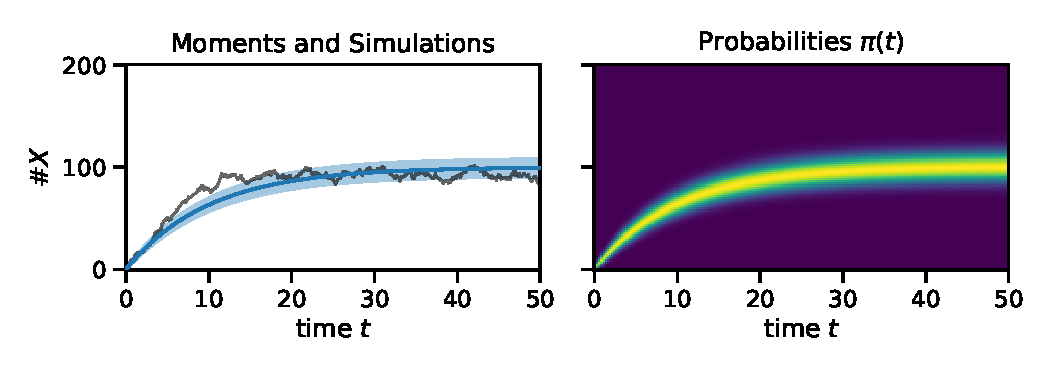
\includegraphics[width=0.9\textwidth]{gfx/momsandprobs.pdf}
	\caption[Moments and probability distribution $\pi(t)$]{\label{fig:momsandprobs}The expected value $\pm$ a standard deviation along with a sampled trajectory (left) and the probability distribution over time (right) of \autoref{model:bd} with $\mu=10$ and $\gamma=0.1$.}
\end{figure}

\section{Stationary Distribution}\label{sec:stationary_dist}
Assuming
% irreducibility and 
ergodicity  
of the underlying chain, a stationary distribution $\pi_{\infty}$ is an invariant distribution, namely a fixed point of the Kolmogorov forward equation \eqref{eq:forward}.
Let $\pi_{\infty}$ be the vector description of a stationary distribution. It then  satisfies
\begin{equation}\label{eq:stationary}
0=\pi_{\infty}Q\quad\text{and}\quad 1=\sum_{x\in\mathcal{S}}\pi_{\infty}(x)
\end{equation}
as a fixed point of the Kolmogorov equation \eqref{eq:forward}.
Stationary distributions are connected to the \emph{long-run} behavior of an \ac{MPM}~\cite{dayar2011bounding}, as the system's distribution will converge to the (unique)
stationary distribution.
The connection of the stationary distribution to the long-run behavior becomes clear when considering the ergodic theorem. 
For some $A\subseteq\mathcal{S}$,
\begin{equation}\label{eq:ergodic}
    \lim_{T\to\infty}\frac{1}{T}\int_0^T 1_A(X_t)\,dt
    = \sum_{x\in A}\pi_{\infty}(x)\,.
\end{equation}
Thus, the mean occupation time for set $A$ over infinite trajectories is the stationary measure for $A$.
Eq.~\eqref{eq:ergodic} shows that we can assess long-run behavior using the stationary distribution and vice-versa.

\paragraph{Example.} Returning to the example of \autoref{model:bd} it is obvious that the state-space is irreducible.
Further, we can easily show, that the stationary distribution is Poissonian with rate $\mu/\gamma$:
$$ \pi_{\infty}(x)=\frac{{(\mu/\gamma)}^{x}\exp(-\mu/\gamma)}{x!}\,.$$


For simplicity, we assume throughout that the state-space is composed of a single communicating class.
Checking ergodicity given a countably infinite number of states is achieved by providing a suitable Foster-Lyapunov function \cite{meyn2012markov}.
Some automated techniques have been proposed for this task \cite{dayar2011bounding,gupta2014scalable,milias2014optimization}.



\subsection{Lyapunov Bounds}\label{sec:statagg:lyapunov}
It is well-known that for a \ac{CTMC} $X$, ergodicity can be proven by a Lyapunov function $g:\mathcal{S}\to\mathbb{R}_+$ \cite{meyn1993stability,dayar2011bounding}.\footnote{The positivity requirement can somewhat be relaxed. The function only needs to be bounded from below since it can be shifted to the positives. In practice this shift can be ignored since it cancels out in the drift \eqref{eq:drift}.}
Given the $g$, we define its \emph{drift} $d$ as its average infinitesimal change, which is obtained applying the generator $Q$ to $g$. 
\begin{equation}\label{eq:drift}
	d(x) = Qg(x) = \sum_{j=1}^{n_R} \alpha_j(x) (g(x+v_j) -  g(x))
\end{equation}
A Lyapunov function can be used to prove ergodicity of a \ac{CTMC}: If there is a finite subset $C\subset\mathcal{S}$ such that
\begin{align}
	&Qg(x)\leq -1,\; \forall x\in\mathcal{S}\setminus C\,,\\
	&Qg(x)< \infty,\; \forall x\in C\,, and\\
	&\lVert x\rVert\to\infty \Rightarrow g(x)\to\infty\,,\;\text{ where }\;\lVert x\rVert=\sum_i x_i\,,
\end{align}
then the chain is non-explosive and ergodic~\cite{milias2014optimization,tweedie_1975}.


Usually, such a function $g$ grows in all directions on the positive orthant, while its drift $d(x)$ decreases in all directions.
More formally, $g$ is characterized by having finite level sets $\{x\in\mathcal{S} \mid g(x) < l\}$ for all $l > 0$.
At the same time,
\begin{equation}\label{eq:lyapunov_set}
    \mathcal{C}_{\epsilon_{\ell}} = \{ x\in\mathcal{S} \mid
    \frac{\epsilon_{\ell}}{c}d(x) > \epsilon_{\ell} - 1\}
\end{equation}
should be finite, where $\infty> c\geq \sup_{x\in\mathcal{S}} d(x)$.
In this case, $\mathcal{C}_{\epsilon_{\ell}}$ contains at least $1-\epsilon_{\ell}$ of stationary probability mass for any $\epsilon_{\ell}\in(0,1)$ \cite[Thm.~8]{spieler2014numerical}.
Given that $\mathcal{C}_{\epsilon_{\ell}}$ is finite, the chain is ergodic and
\begin{equation}
    \sum_{x\in\mathcal{C}_{\epsilon_{\ell}}}\pi(x)> 1 - \epsilon_{\ell}
\end{equation}
bounding the stationary probability mass contained within $\mathcal{C}_{\epsilon_{\ell}}$.



\section{A Brief Taxonomy of Multimodality}\label{sec:multimodality}
Multimodality is an overloaded term in the context of reaction network models.
Specifically, it can be used to describe the following features.
\begin{description}
	\item[Operational Multimodality]
		This kind of multimodality characterizes the model behavior directly.
		Consider, for example, a gene
		expression model\marginpar{\autoref{model:gexpr}
		on page~\pageref{model:gexpr} is an instance of this.}:
		The gene state is digital, meaning it is either active or inactive.
		Depending on this state a protein is either synthesized or not.
		Therefore the system has distinct \emph{operational modes}
		which dictate its dynamics.
		Non-biological examples can be found in the
		context of broadcasting systems,
		in which the dynamics change discretely due to messages shared between
		agents~\cite{bortolussi2020fluid}.

		Naturally, nearly all models change their dynamics,
		given a change in their state vector.
		In this aspect this distinction is not wholly strict.
		It is mainly intended to indicate distinctive changes in the dynamics.
		In some instances, these can be as obvious as the examples mentioned above.
		In other cases they may not be as obvious:
		Consider an epidemics die-out for example, which is a significant change
		in the operating mode, which is not due to a switch-type reaction.
  \item[Distributional Multimodality]
	  Here the multimodality refers to the stationary distribution $\pi_{\infty}$:
		It has multiple
		\emph{modes}, i.e.\ local maxima. Given an ergodic underlying \ac{CTMC}
		this entails, that the system spends most time in distinct regions of the
		state-space (cf.\ \eqref{eq:ergodic}).
		The \emph{switching} between those distinct region is of interest
		for both, analysis and control, of such models.
\end{description}
While distributional multimodality implies operational multimodality, the reverse
does not hold.

Literature:
\begin{itemize}
	\item \cite{siegal2011emergence}
\end{itemize}
